\documentclass[
 size=14pt,
 paper=smartboard,  %a4paper, smartboard, screen
 mode=present, 		%present, handout, print
 display=slides, 	% slidesnotes, notes, slides
 style=tuliplab,  	% TULIP Lab style
 pauseslide,
 fleqn,leqno]{powerdot}


\usepackage{cancel}
\usepackage{caption}
\usepackage{stackengine}
\usepackage{smartdiagram}
\usepackage{attrib}
\usepackage{amssymb}
\usepackage{amsmath} 
\usepackage{amsthm} 
\usepackage{mathtools}
\usepackage{rotating}
\usepackage{graphicx}
\usepackage{boxedminipage}
\usepackage{rotate}
\usepackage{calc}
\usepackage[absolute]{textpos}
\usepackage{psfrag,overpic}
\usepackage{fouriernc}
\usepackage{pstricks,pst-3d,pst-grad,pstricks-add,pst-text,pst-node,pst-tree}
\usepackage{moreverb,epsfig,subfigure}
\usepackage{color}
\usepackage{booktabs}
\usepackage{etex}
\usepackage{breqn}
\usepackage{multirow}
\usepackage{natbib}
\usepackage{bibentry}
\usepackage{gitinfo2}
\usepackage{siunitx}
\usepackage{nicefrac}
%\usepackage{geometry}
%\geometry{verbose,letterpaper}
\usepackage{media9}
\usepackage{animate}
%\usepackage{movie15}
\usepackage{auto-pst-pdf}

\usepackage{breakurl}
\usepackage{fontawesome}
\usepackage{xcolor}
\usepackage{multicol}



\usepackage{verbatim}
\usepackage[utf8]{inputenc}
%\usepackage{dtk-logos}
\usepackage{tikz}
\usepackage{adigraph}
\usepackage{tkz-graph}
\usepackage{hyperref}
\usepackage{ulem}
\usepackage{pgfplots}
\usepackage{verbatim}
\usepackage{fontawesome}


\usepackage{todonotes}
% \usepackage{pst-rel-points}
\usepackage{animate}
\usepackage{fontawesome}

\usepackage{listings}
\lstset{frameround=fttt,
frame=trBL,
stringstyle=\ttfamily,
backgroundcolor=\color{yellow!20},
basicstyle=\footnotesize\ttfamily}
\lstnewenvironment{code}{
\lstset{frame=single,escapeinside=`',
backgroundcolor=\color{yellow!20},
basicstyle=\footnotesize\ttfamily}
}{}


\usepackage{hyperref}
\hypersetup{ % TODO: PDF meta Data
  pdftitle={Presentation Title},
  pdfauthor={Gang Li},
  pdfpagemode={FullScreen},
  pdfborder={0 0 0}
}

\definecolor{LightGray}{rgb}{0.9,0.9,0.9}
\newlength{\pixel}\setlength\pixel{0.000714285714\slidewidth}
\setlength{\TPHorizModule}{\slidewidth}
\setlength{\TPVertModule}{\slideheight}
\newcommand\highlight[1]{\fbox{#1}}
\newcommand\icite[1]{{\footnotesize [#1]}}

\newcommand\twotonebox[2]{\fcolorbox{pdcolor2}{pdcolor2}
{#1\vphantom{#2}}\fcolorbox{pdcolor2}{white}{#2\vphantom{#1}}}
\newcommand\twotoneboxo[2]{\fcolorbox{pdcolor2}{pdcolor2}
{#1}\fcolorbox{pdcolor2}{white}{#2}}
\newcommand\vpspace[1]{\vphantom{\vspace{#1}}}
\newcommand\hpspace[1]{\hphantom{\hspace{#1}}}
\newcommand\COMMENT[1]{}

\newcommand\placepos[3]{\hbox to\z@{\kern#1
        \raisebox{-#2}[\z@][\z@]{#3}\hss}\ignorespaces}

\renewcommand{\baselinestretch}{1.2}


\newcommand{\draftnote}[3]{
	\todo[author=#2,color=#1!30,size=\footnotesize]{\textsf{#3}}	}
% TODO: add yourself here:
%
\newcommand{\gangli}[1]{\draftnote{blue}{GLi:}{#1}}
\newcommand{\shaoni}[1]{\draftnote{green}{sn:}{#1}}
\newcommand{\gliMarker}
	{\todo[author=GLi,size=\tiny,inline,color=blue!40]
	{Gang Li has worked up to here.}}
\newcommand{\snMarker}
	{\todo[author=Sn,size=\tiny,inline,color=green!40]
	{Shaoni has worked up to here.}}

%%%%%%%%%%%%%%%%%%%%%%%%%%%%%%%%%%%%%%%%%%%%%%%%%%%%%%%%%%%%%%%%%%%%%%%%
% title
% TODO: Customize to your Own Title, Name, Address
%
\title{Ordinal Regression with a Tabular Wine Quality Dataset}
\author{
Sen Han, Gang Li
\\Beijing Technology and Business University
\\Deakin University
}
\date{\gitCommitterDate}


% Customize the setting of slides
\pdsetup{
% TODO: Customize the left footer, and right footer
rf=\href{http://www.tulip.org.au}{
Last Changed by: \textsc{\gitCommitterName}\ (\gitAuthorDate)
},
cf={Ordinal Regression with a Tabular Wine Quality Dataset},
}
%' \gitVtagn-\gitAbbrevHash\ '

\begin{document}

\maketitle

%\begin{slide}{Overview}
%\tableofcontents[content=sections]
%\end{slide}


%%==========================================================================================
%%
\begin{slide}[toc=,bm=]{Overview}
\tableofcontents[content=currentsection,type=1]
\end{slide}
%%
%%==========================================================================================


\section{Introduction}

%%==========================================================================================

\begin{slide}{Problem Description}
	\begin{center}
		\twotonebox{\rotatebox{90}{Defn}}{\parbox{.86\textwidth}{
				Ordinal regression was conducted on a dataset derived from a deep learning model trained on the quality dataset of red variants of the "Vinho Verde" wine from Spain. This dataset characterizes the impact of various chemical substances present in wine on its quality. The quality grades are ordinal and imbalanced, with common wines being significantly more prevalent than either high-quality or low-quality wines.}}
	\end{center}
\end{slide}

%%==========================================================================================

\begin{slide}{Dataset Description}
	\begin{center}
		\twotonebox{\rotatebox{90}{Wine Quality}}{\parbox{.86\textwidth}
			{This datasets is related to red variants of the Portuguese "Vinho Verde" wine.The dataset describes the amount of various chemicals present in wine and their effect on it's quality. The datasets can be viewed as classification or regression tasks. The classes are ordered and not balanced (e.g. there are much more normal wines than excellent or poor ones).Your task is to predict the quality of wine using the given data.
		}}
		
	\end{center}
\end{slide}
%%
%%==========================================================================================

\section{Preliminaries}

%%==========================================================================================
\begin{slide}{Wine Features}

In order to facilitate an understanding of the meanings of various data points in the dataset, it is necessary to provide a brief introduction to several features of wine that are relevant to the dataset.
	\begin{itemize}
	\item \textbf{Fixed acidity:} Most acids involved with wine or fixed or nonvolatile (do not evaporate readily).
	\item \textbf{Volatile acidity:} The amount of acetic acid in wine, which at too high of levels can lead to an unpleasant, vinegar taste.
	\item \textbf{Citric acid:} Found in small quantities, citric acid can add 'freshness' and flavor to wines.
	\item \textbf{Residual sugar:} The amount of sugar remaining after fermentation stops, it's rare to find wines with less than 1 gram/liter and wines with greater than 45 grams/liter are considered sweet.
	SS
\end{itemize}
	
\end{slide}

%%==========================================================================================

\begin{slide}[toc=]{Wine Features}
	
	\begin{itemize}
	
		\item \textbf{Chlorides:} The amount of salt in the wine.
		\item \textbf{Free sulfur dioxide:} The free form of SO2 exists in equilibrium between molecular SO2 (as a dissolved gas) and bisulfite ion; it prevents microbial growth and the oxidation of wine.
		\item \textbf{Total sulfur dioxide:} Amount of free and bound forms of S02; in low concentrations, SO2 is mostly undetectable in wine, but at free SO2 concentrations over 50 ppm, SO2 becomes evident in the nose and taste of wine.
		\item \textbf{Density:} The density of water is close to that of water depending on the percent alcohol and sugar content.
		\item \textbf{pH:} Describes how acidic or basic a wine is on a scale from 0 (very acidic) to 14 (very basic); most wines are between 3-4 on the pH scale.
		\item \textbf{Sulphates:} A wine additive which can contribute to sulfur dioxide gas (S02) levels, which acts as an antimicrobial and antioxidant.
		\item \textbf{Alcohol:} The percent alcohol content of the wine.
		\item \textbf{Quality:} Wine quality rating.
	\end{itemize}
	
\end{slide}
%%==========================================================================================
\begin{slide}{SMOTE}
	
	\begin{itemize}
		\item \textbf{Data Imbalance in Dataset:} In the provided dataset, the samples with quality grades 5 and 6 are substantially more numerous than those of other grades, necessitating a consideration of the potential impacts of employing the SMOTE technique.
		
		\item \textbf{What is SMOTE?} SMOTE (Synthetic Minority Over-sampling Technique) is a method employed in data science and machine learning to address the issue of class imbalance in classification problems. Class imbalance refers to the scenario where the instance count of one class (the minority class) is significantly lower than that of other classes (the majority classes). 
		
		\item \textbf{Impact on Machine Learning:} This imbalance can lead to biased performance or suboptimal results in machine learning models, as they are often dominated by the majority class and tend to overlook the minority class.
		
		\item \textbf{Benefits of SMOTE:} By generating synthetic samples, SMOTE aids in reducing the overfitting issues that simple over-sampling might cause.
	\end{itemize}
	
\end{slide}
%%==========================================================================================
\begin{slide}{Scoring Method}
	\begin{itemize}
		\small 
		\item Submissions are scored on the \textbf{quadratic weighted kappa}, which measures agreement between two ratings.
		\item This metric varies from 0 (random agreement) to 1 (complete agreement). It may be negative if there is less agreement than chance.
		\item The calculation involves several steps:
		\begin{enumerate}
			\item Construct an \( N \times N \) histogram matrix \( O \) where \( O_{i,j} \) is the number of agreements between raters.
			\item Calculate a weight matrix \( w \) as follows:
			\[
			w_{i,j} = \frac{(i - j)^2}{(N - 1)^2}
			\]
			\item Calculate the expected outcome matrix \( E \), assuming no correlation as the outer product of sums of \( O \).
			\item The \textbf{quadratic weighted kappa} is then:
			\[
			\kappa = 1 - \frac{\sum w_{i,j} O_{i,j}}{\sum w_{i,j} E_{i,j}}
			\]
		\end{enumerate}
	\end{itemize}
\end{slide}
%%==========================================================================================
\section{Experiment and analysis}
%%==========================================================================================
\begin{slide}{Dataset Analysis}
	\begin{itemize}
		\item Analysis of the Original Dataset, Training Dataset, and Testing Dataset
		\item Null Value Detection
		
		The datasets do not contain any missing values, thus negating the necessity for missing value processing.
	\end{itemize}
\begin{center}
	\includegraphics[width=0.8\textwidth]{tex/NullValueDetection}
\end{center}

\end{slide}


%%==========================================================================================
\begin{slide}[toc=]{Dataset Analysis}
	\begin{itemize}
		\item Target Variable Analysis
	\end{itemize}
\begin{center}
	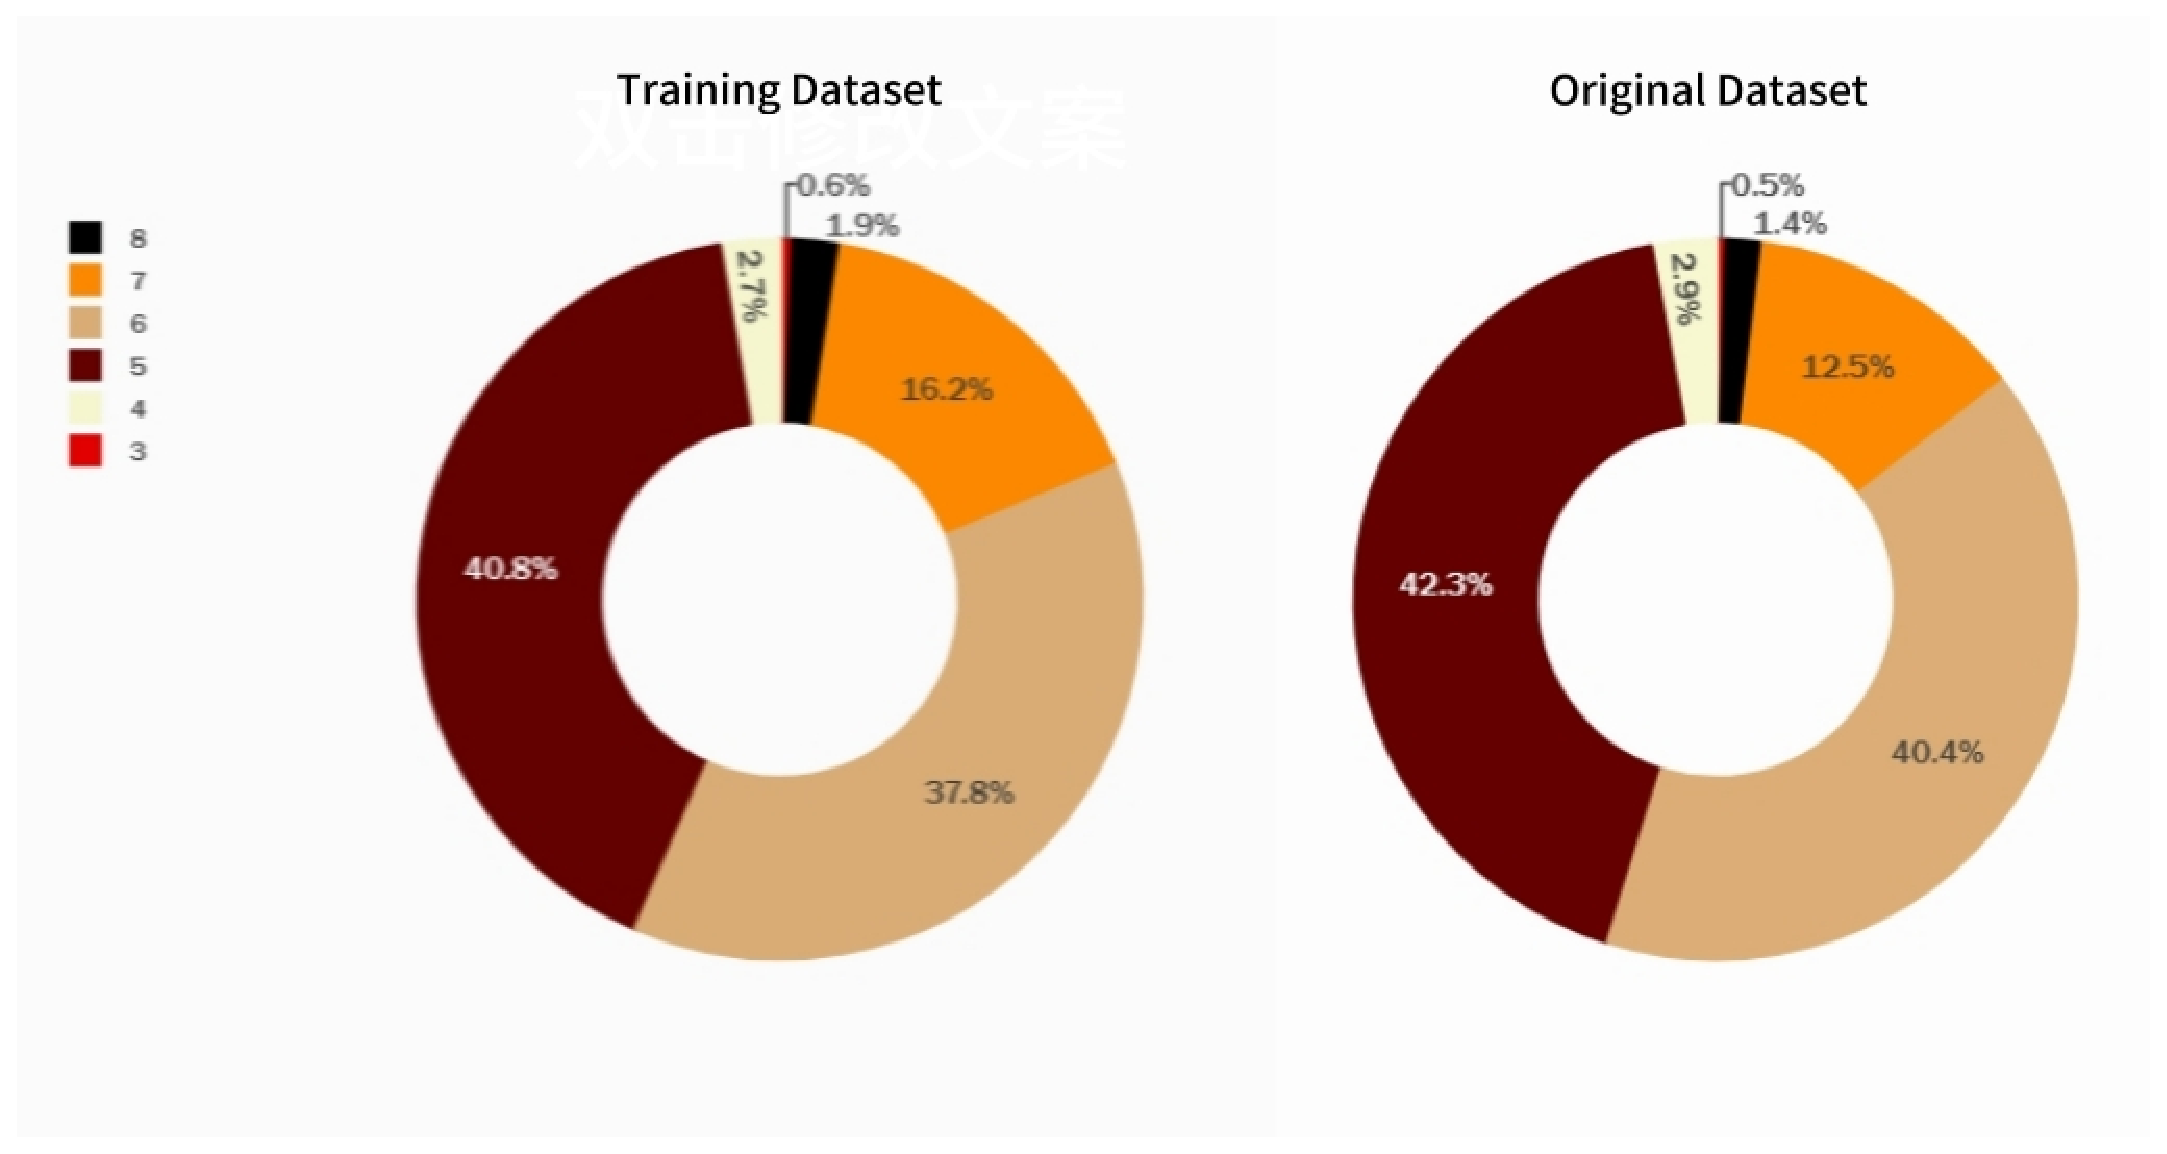
\includegraphics[width=\textwidth]{tex/TargetVariableAnalysis}
\end{center}

\end{slide}


%%==========================================================================================
\begin{slide}[toc=]{Dataset Analysis}
	\begin{itemize}
		\item Univariate Analysis
	\end{itemize}
\begin{center}
	\includegraphics[width=\textwidth]{tex/UnivariateAnalysis}
\end{center}
	
\end{slide}

%%==========================================================================================
\begin{slide}[toc=]{Dataset Analysis}
	For all three datasets, the distributions are almost identical, thus enabling the amalgamation of the original dataset with the training dataset for the purpose of training.
	
	
\end{slide}
%%==========================================================================================
\begin{slide}[toc=]{Combining Data and Relationship Matrix}
	\begin{itemize}
		\item Merged the original dataset with the training dataset to create a combined training dataset.
		\item Calculated the pairwise Spearman correlation coefficients for all numerical columns in the dataset and visualized them in a matrix form.
	\end{itemize}

\begin{minipage}[c]{0.48\textwidth}
	The heatmap below illustrates the monotonic relationship between pairs of variables, using a color scale to signify the strength of the correlation. Darker shades represent stronger correlations, with one color for positive and another for negative correlations. The numerical values in the heatmap's cells indicate the Spearman correlation coefficients for the features they intersect.
\end{minipage}
\hfill
\begin{minipage}[c]{0.48\textwidth}
		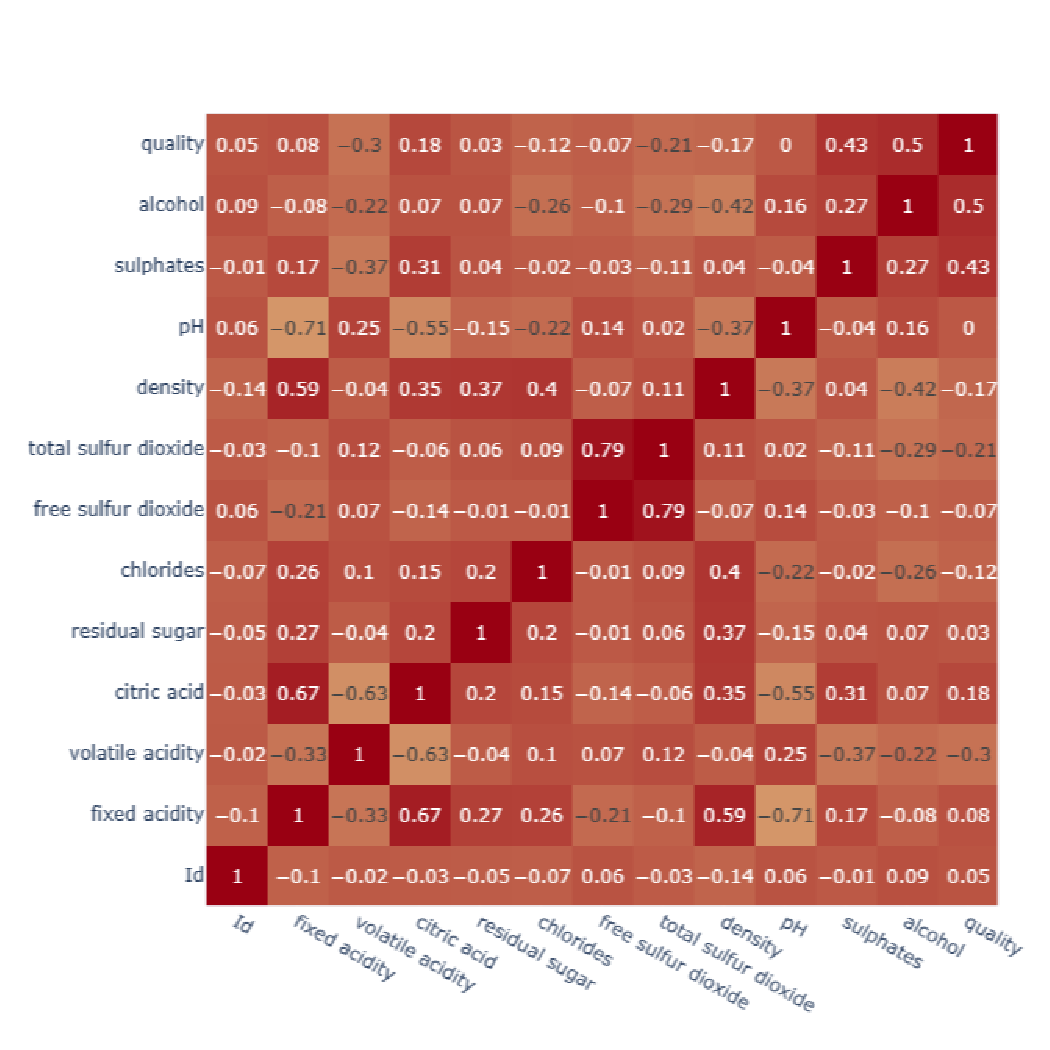
\includegraphics[width=0.9\textwidth]{tex/CombinedTrainingDataset}
\end{minipage}
\end{slide}
%%==========================================================================================
\begin{slide}[toc=]{Multivariate Analysis wrt Quality}
	\begin{minipage}[t]{0.48\textwidth}
		Relation with Quality using pairplot (Combined Training and Original Data)
		
		\smallskip
		
		Analyzing the relationship between various features and the wine quality through visual methods provides insightful observations:
		
		\begin{itemize}
			\item Higher alcohol content tends to correspond with higher quality ratings.
			\item Lower volatile acidity is often associated with higher quality wines.
			\item A higher sulphate content might indicate a trend towards higher quality.
		\end{itemize}
		
		Such visual analyses are pivotal in understanding the influence of individual components on the overall quality of wine.
	\end{minipage}
	\hfill
	\begin{minipage}[t]{0.48\textwidth}
		\centering
		\begin{figure}
			\centering
			\includegraphics[width=0.9\linewidth]{tex/pairplot}
		\end{figure}
	\end{minipage}
\end{slide}
%%==========================================================================================
\begin{slide}[toc=]{Relation with Quality using Boxplot}
	\begin{minipage}{0.5\textwidth}
		
			\textbf{Combined Training and Original Data Analysis:}
			
			Through boxplots, we can observe the distribution of features across different quality levels. Key insights include:
			
			\begin{itemize}
				\item Higher-quality wines have higher medians in sulphates, alcohol, and citric acid.
				\item Conversely, they have lower medians in chlorides, density, and residual sugar.
			\end{itemize}
			
			These observations can guide further analysis and predictive modeling.
	\end{minipage}%
	\hfill
	\begin{minipage}{0.45\textwidth}
		\centering
		\begin{figure}
			\centering
			\includegraphics[width=1\linewidth]{tex/boxplot}
		\end{figure}
		
	\end{minipage}
\end{slide}
%%==========================================================================================
\begin{slide}{Analysis So Far}
	\begin{itemize}
		\item The distribution of data points across the training, testing, and original datasets is approximately the same, suggesting consistency in data collection or generation.
		\item The relationships between variables show similar patterns in both the test set and the combined dataset (which includes training and original data), indicating that the test set may be a representative subset of the overall data.
	\end{itemize}
\end{slide}
%%==========================================================================================
\begin{slide}[toc=]{Data Preparation: Normal vs SMOTE}
	\begin{minipage}[t]{0.48\textwidth}
		\textbf{Regular Training Data}
		\begin{itemize}
			\item Class distribution in the combined training dataset shows imbalance:
			
			\begin{tabular}{lc}
				\textbf{Quality} & \textbf{Count} \\
				\hline
				5 & 925 \\
				6 & 868 \\
				7 & 333 \\
				4 & 62  \\
				8 & 38  \\
				3 & 13  \\
			\end{tabular}
		\end{itemize}
	\end{minipage}
	\hfill
	\begin{minipage}[t]{0.48\textwidth}
		\textbf{SMOTE Training Data}
		\begin{itemize}
			\item After applying SMOTE, class distribution is balanced:
			
			\begin{tabular}{lc}
				\textbf{Quality} & \textbf{Count} \\
				\hline
				3 & 925 \\
				4 & 925 \\
				5 & 925 \\
				6 & 925 \\
				7 & 925 \\
				8 & 925 \\
			\end{tabular}
		\end{itemize}
	\end{minipage}
\end{slide}
%%==========================================================================================
\begin{slide}{Classification Approach}
	
	\begin{minipage}[c]{0.5\textwidth}
		% 文本内容放在这里
		Train various models separately on 70\% of the data randomly drawn from both the combined training dataset and the SMOTE-enhanced training dataset. Then test these models on the remaining 30\% of the data to calculate their respective Kappa scores.
	\end{minipage}
	\hfill
	\begin{minipage}[c]{0.45\textwidth}
		% 图像代码放在这里
\begin{center}
	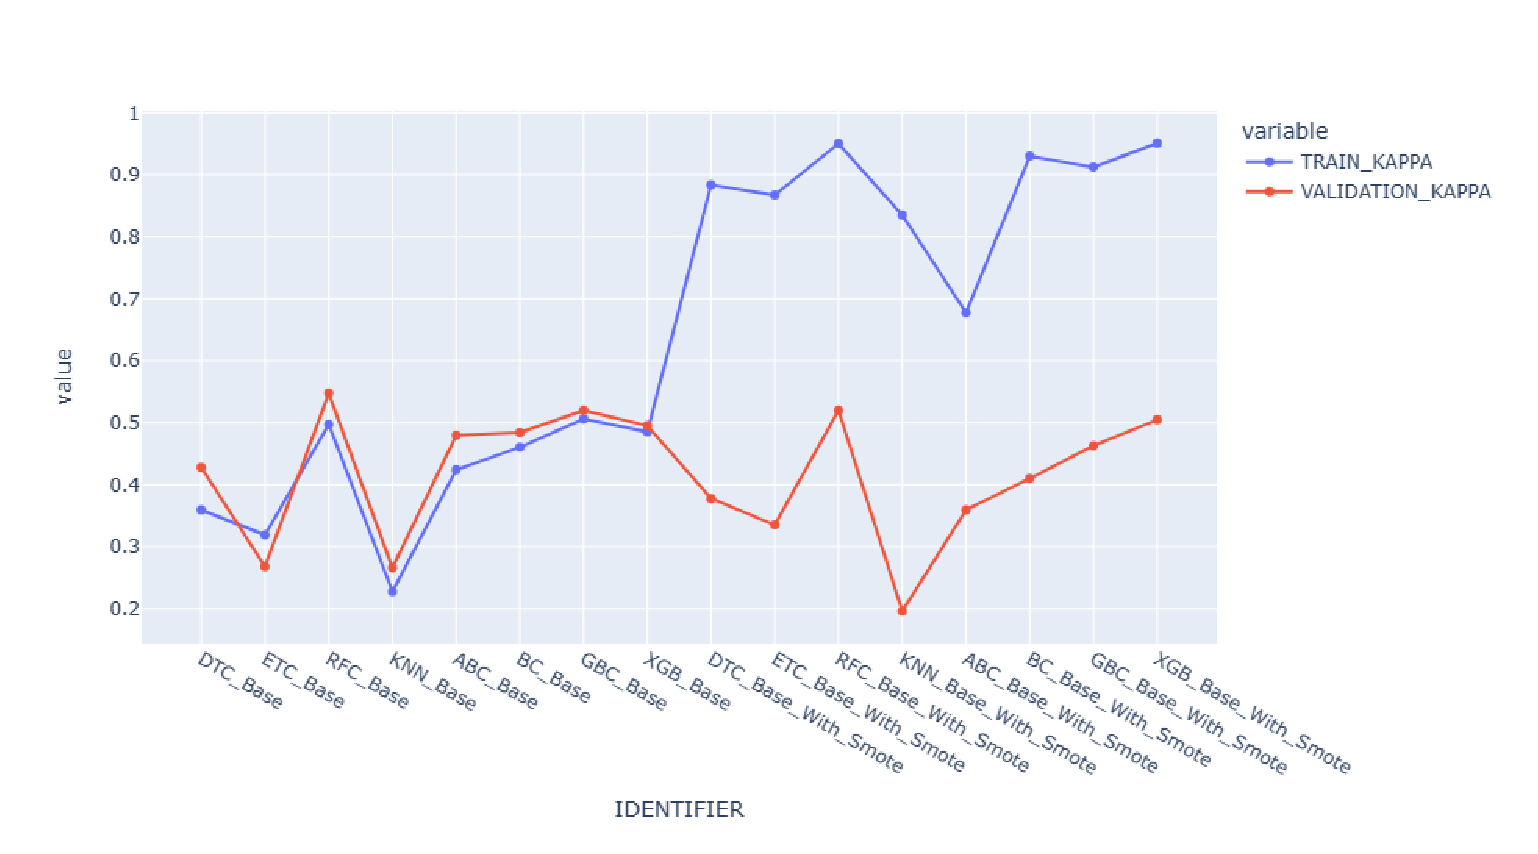
\includegraphics[width=\textwidth]{tex/kappa}
\end{center}
	\end{minipage}
	
\end{slide}

%%==========================================================================================

\section{Conclusion}

%%==========================================================================================

\begin{slide}[toc=]{Conclusion}
	\begin{center} 
		In scenarios where models are trained using both the combined training dataset and the SMOTE-enhanced training dataset, it appears that there is no significant difference in performance on the validation set. However, the use of the SMOTE-enhanced dataset seems to improve model performance on the training set. This indicates that the application of the SMOTE technique may aid in better fitting the model to the training data, particularly when dealing with class imbalances in datasets.
	\end{center}
\end{slide}

%%==========================================================================================

\section{Submission}

%%==========================================================================================

\begin{slide}[toc=]{Submission}
	
	\begin{itemize}
		\item After an extensive evaluation of different models under various conditions,
		\item the Random Forest, Light Gradient Boosting Machine, and Gradient Boosting Classifier have been chosen.
		\item These models will be applied to the test dataset for ordinal regression using a voting mechanism (mode),
		\item and the predictions will be exported to a file named \texttt{xyz.csv}.
	\end{itemize}
	
\end{slide}

%%==========================================================================================

\section{Acknowledgement}

%%==========================================================================================
\begin{slide}[toc=]{Acknowledgement}
	
	I would like to express my sincere gratitude to Zhang Baojie, Wang Tianjiao, and Li Leyan for their invaluable support during my learning journey. Their assistance has been instrumental in overcoming the challenges faced along the way.
	
\end{slide}

%%==========================================================================================


\begin{wideslide}[toc=,bm=]{Contact Information}
\centering
\vspace{\stretch{1}}
\twocolumn[
lcolwidth=0.35\linewidth,
rcolwidth=0.65\linewidth
]
{
% \centerline{\includegraphics[scale=.2]{tulip-logo.eps}}
}
{
\vspace{\stretch{1}}
Associate Professor Gang Li\\
School of Information Technology\\
Deakin University, Australia
\begin{description}
 \item[\textcolor{orange}{\faEnvelope}] \href{mailto:gangli@tulip.org.au}
 {\textsc{\footnotesize{gangli@tulip.org.au}}}

 \item[\textcolor{orange}{\faHome}] \href{http://www.tulip.org.au}
 {\textsc{\footnotesize{Team for Universal Learning and Intelligent Processing}}}
\end{description}
}
\vspace{\stretch{1}}
\end{wideslide}

\end{document}

\endinput
